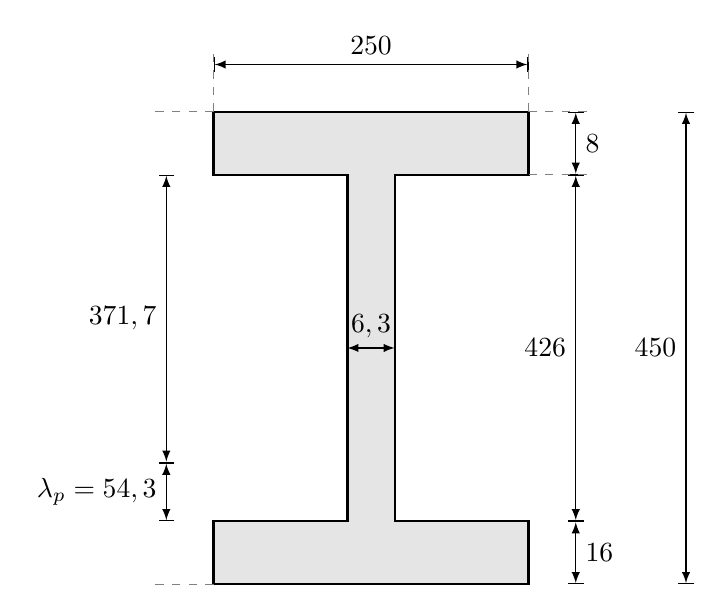
\begin{tikzpicture}[
    % Configuração global das setas de cota para ficarem com aparência técnica
    cota/.style={|<->|, >=latex, thin},
    % Estilo da linha do perfil
    perfil/.style={thick, fill=gray!20, draw=black}
]

    % ==========================================
    % 1. DESENHANDO O PERFIL I (Coordenadas)
    % ==========================================
    % Consideraremos as seguintes medidas base para o desenho:
    % Largura da mesa (bf) = 4cm (de x=-2 até x=2)
    % Altura total (d) = 6cm (de y=0 até y=6)
    % Espessura da mesa (tf) = 0.8cm
    % Espessura da alma (tw) = 0.6cm (de x=-0.3 a x=0.3)
    
    \draw[perfil] 
        (-2, 0) -- (2, 0)          % Base inferior
        -- (2, 0.8)                % Sobe a lateral direita da mesa inferior
        -- (0.3, 0.8)              % Entra em direção à alma
        -- (0.3, 5.2)              % Sobe a alma pelo lado direito
        -- (2, 5.2)                % Sai para a direita na mesa superior
        -- (2, 6)                  % Sobe a lateral direita da mesa superior
        -- (-2, 6)                 % Topo superior
        -- (-2, 5.2)               % Desce a lateral esquerda da mesa superior
        -- (-0.3, 5.2)             % Entra em direção à alma
        -- (-0.3, 0.8)             % Desce a alma pelo lado esquerdo
        -- (-2, 0.8)               % Sai para a esquerda na mesa inferior
        -- cycle;                  % Fecha o caminho de volta ao (-2,0)


    % ==========================================
    % 2. DESENHANDO AS COTAS (Linhas de dimensão)
    % ==========================================
    % O comando node[posiçao] coloca o texto alinhado à linha [1]
    
    % Cota da Altura Total (d) - Lado esquerdo
    \draw[cota] (4, 0) -- node[left] {$450$} (4, 6);
    \draw[cota] (2.6, 0.8) -- node[left] {$426$} (2.6, 6-0.8);
    \draw[cota] (-2.6, 1.543) -- node[left] {$371,7$} (-2.6, 6-0.8);
    \draw[cota] (-2.6, 0.8) -- node[left] {$\lambda_p = 54,3$} (-2.6, 1.543);
    % Linhas auxiliares pontilhadas para a altura
    \draw[dashed, gray] (-2, 6) -- (-2.8, 6);
    \draw[dashed, gray] (-2, 0) -- (-2.8, 0);

    % Cota da Largura da Mesa (bf) - Topo
    \draw[cota] (-2, 6.6) -- node[above] {$250$} (2, 6.6);
    % Linhas auxiliares pontilhadas para a largura
    \draw[dashed, gray] (-2, 6) -- (-2, 6.8);
    \draw[dashed, gray] (2, 6) -- (2, 6.8);

    % Cota da Espessura da Mesa (tf) - Lado direito
    \draw[cota] (2.6, 5.2) -- node[right] {$8$} (2.6, 6);
    \draw[cota] (2.6, 0) -- node[right] {$16$} (2.6, 0.8);
    % Linhas auxiliares pontilhadas para tf
    \draw[dashed, gray] (2, 6) -- (2.8, 6);
    \draw[dashed, gray] (2, 5.2) -- (2.8, 5.2);

    % Cota da Espessura da Alma (tw) - Centro
    % Como o espaço é pequeno, não usamos o |<->|, usamos apenas <->
    \draw[<->, >=latex, thin] (-0.3, 3) -- node[above] {$6,3$} (0.3, 3);

\end{tikzpicture}